\chapter{Planificación}\label{cap:planif}
%\minitoc

\section{Requisitos}
[Sobre todo en proyectos de diseño software/hardware]

\section{Tareas}
[A partir de los objetivos planteados del proyecto se definirán tareas así como su duración. Un objetivo, puede dar lugar a más de una tarea para su consecución. Es importante relacionar cada tarea con sus objetivos asociados.]

\begin{itemize}
    \item \textbf{Estudio del estado del arte.} ...
    \item \textbf{Evaluación de la propuesta} 
\end{itemize}

\section{Recursos humanos y técnicos}

Los recursos necesitamos para llevar a cabo el proyecto son:

\begin{itemize}
    \item \textbf{Hardware}:
    
    \begin{itemize}
        \item Ordenador de sobremesa HP Z2 SFF G4 Workstation del Laboratorio de Ciberseguridad de la UGR.
        
        \item ...
    \end{itemize}
        
    \item \textbf{Software}:
        
    \begin{itemize}
        \item Sistema operativo Ubuntu 18.04 LTS. Será la distribución Linux principal con la que vamos a trabajar, tanto en forma nativa como en máquinas virtuales.
        
        \item ...
        
    \end{itemize}
    
    \item \textbf{Recursos humanos}. En la Tabla~\ref{table:recursos-humanos} se muestra una aproximación de las horas de trabajo empleadas en las diferentes tareas realizadas, tanto por el desarrollador como por el supervisor, incluyendo las reuniones asociadas a cada tarea.
\end{itemize}

\section{Temporización}

Para alcanzar los objetivos de cualquier proyecto, es necesario llevar a cabo una planificación temporal de las diferentes tareas a realizar.

En nuestro caso, no hemos dispuesto de todos los recursos desde el primer momento, por lo que hemos ido adaptando las tareas conforme a lo que podíamos llevar a cabo. La duración de cada tarea depende de varias aspectos como su complejidad y disposición de recursos.

Las diferentes tareas que hemos llevado a cabo las mostramos en el diagrama de Gantt donde hemos realizado una planificación por semanas (ver Figura~\ref{fig:gantt}).

Para controlar que estas tareas se cumplen en los plazos establecidos, se han llevado a cabo diferentes reuniones con el tutor en las cuales se exponía el trabajo realizado y se determinaban las siguientes tareas a llevar a cabo.

\begin{table}[t!]
\begin{tabular}{|c|c|c|}
\hline
\textbf{Tarea} & \textbf{\begin{tabular}[c]{@{}c@{}}Tiempo empleado \\ por el \\ desarrollador (horas)\end{tabular}} & \textbf{\begin{tabular}[c]{@{}c@{}}Tiempo empleado \\ por el \\ tutor (horas)\end{tabular}} \\ \hline
Estado del arte & 25 & 5 \\ \hline
Análisis de las soluciones & 30 & 7 \\ \hline
Diseño e implementación & 60 & 6 \\ \hline
Evaluación de seguridad & 20 & 5 \\ \hline
Securización del sistema & 15 & 2 \\ \hline
\textbf{Total} & \textbf{150} & \textbf{25} \\ \hline
\end{tabular}
\caption{Resumen recursos humanos.}
\label{table:recursos-humanos}
\end{table}

\begin{figure}[t!]
    \centering
    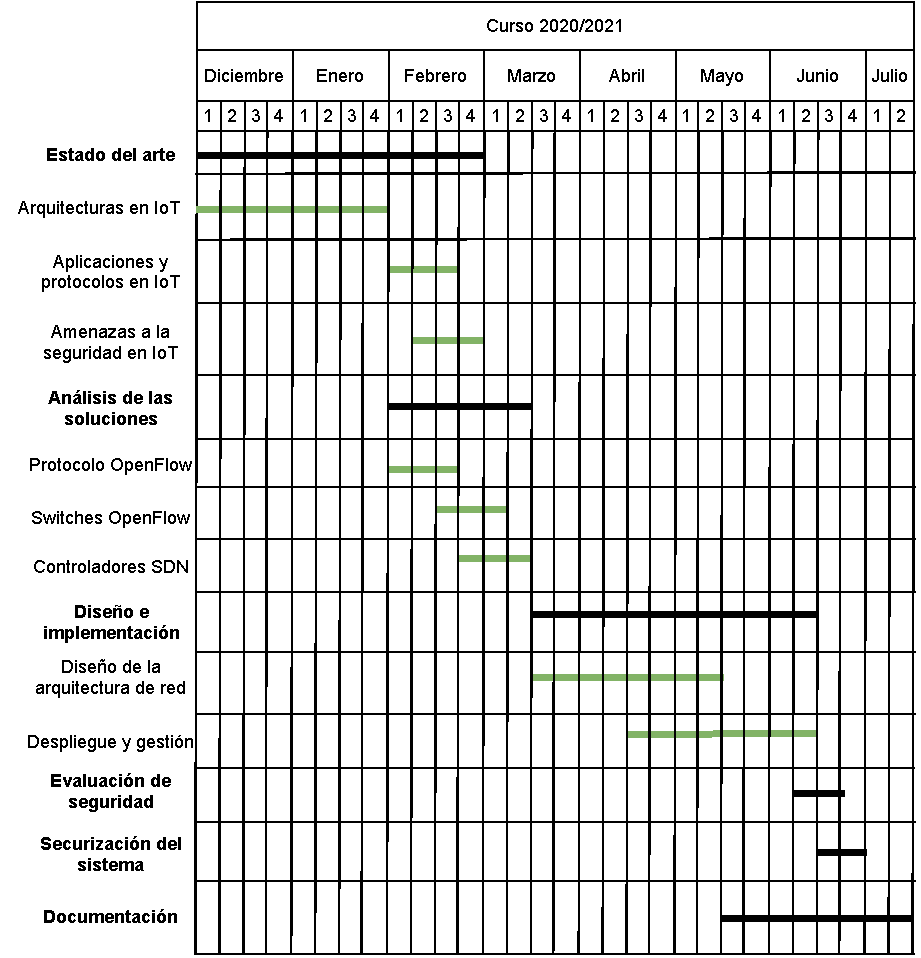
\includegraphics[width=1\textwidth]{imagenes/cap2/gannt.pdf}
    \caption{Diagrama de Gantt del proyecto.}
    \label{fig:gantt}
\end{figure}